\documentclass[output=paper]{langsci/langscibook}
\ChapterDOI{10.5281/zenodo.573776}

\author{Jeremy Collins\affiliation{Radboud University, Nijmegen}}
\title{Real and spurious correlations involving tonal languages} 
\maketitle
\begin{document}

\is{tone} \is{cultural adaptation} \noindent Why are some languages tonal?  Is there a fundamental reason why some languages develop tone and others do not, and and does this have an effect on the way the rest of the language is organized?  Tone is important in the context of dependencies, because there is no shortage of hypotheses about what can cause tone and what else tone can cause.  For example, tonal languages are found predominantly in warm, humid climates, suggesting that they are culturally adaptive in those environments \citep{Everett2015}; they are also found in places with low frequencies of two genes microcephalin and ASPM, suggesting that some populations are more likely to use tone than others because of their genetics \citep{Dediu2007}.  One paper furthermore proposed that phoneme diversity declines with distance from Africa, and number of tones in particular, suggesting a founder effect of migrations, as well as a link with modern population size \citep{Atkinson2011}.  As for effects on the rest of the language, SVO word order \citep{Yiu2013} and various other grammatical \is{constituent order} properties have been suggested to linked functionally with tone, and by \citet{Donegan1983} in particular for languages in the \ili{Austro-Asiatic} family.

%As for effects on the rest of the language, SVO word order \citep{Yiu2013} and various other grammatical properties have been suggested to linked functionally with tone, and by \citet{Donegan1983} in particular for languages in the within \ili{Austro-Asiatic} family.



\is{African languages} \is{Southeast Asian languages} \is{serial verb constructions} At least part of the reason for the large number of correlations proposed in the literature is the visibly skewed geographical distribution of tonal languages (\figref{fig:collins:1}). They are predominantly found in Africa and Southeast Asia, immediately suggesting that tone will correlate with a large number of things, from humid climates and SVO languages, to serial verbs, and ancient settlement.  The map of ASPM and microcephalin in particular, by Dediu and Ladd’s own admission, was the inspiration for their correlation, when they saw that it was similar to the map of tonal languages.  But by a similar reasoning, tone can be linked in a spurious way with other things found in those regions, such as acacia trees \citep{Roberts2013}.  It is therefore necessary to work out a way to distinguish which of these correlations are real, and which of these are merely accidental consequences of these cultural traits being spatially auto-correlated.  



\is{tone} A further major obstacle is the fact that tonal languages are typically not independent.  Whole large language families can be tonal, such as \ili{Niger-Congo} and \ili{Sino-Tibetan}.  The influence of these families in Africa and Southeast Asia has furthermore caused many languages in those regions to become tonal as well, if they were not already due to ancient relatedness with other tonal families \citep{EnfieldAreal2005}.  If one wants to demonstrate that tone correlates with anything, then one in principle has to use independent data points, which may prove impossible in practice.



I focus in this paper on the correlation proposed by \is{ASPM} \is{microcephalin} \is{Mantel testing} \citeauthor{Dediu2007} with ASPM and microcephalin, and briefly discuss the correlation proposed by  \citeauthor{Everett2015} with humidity, based on my response to their paper \citep{CollinsInPress}. My assessment of their causal claims will be primarily negative.  The reasons I give will be that the evidence for their causal mechanisms are inadequate, and that the methods that they claim control for language family and geographical distance do not work.  These points have broader relevance than just for tone, as these affect the way that correlations in general are studied typologically, a point also emphasized by recent work by \citet{Ladd2015}. I end the paper with some broader points illustrating the way that the problem of non-independence in linguistics can take some subtle forms, complicating the search for the genuine dependencies which exist in linguistic systems.



\section{Tone and genes}



\citet{Dediu2007} argue that two genes, ASPM and Microcephalin, may have an effect on the processing of tone.  Speakers with particular alleles of these genes are found in regions where tonal languages are.  The correlation between these genes and tone is strong (stronger than 97.3\% of all gene-language correlations that they tested), and it remains significant in a partial Mantel test controlling for language relatedness and distance between languages.  Since these two genes are expressed in the brain, the reason for this may be that these two genes have an effect on speakers’ processing of tone, causing some languages to be less likely to develop tone than others, given that there are large differences between populations in the frequency of these genes.  



This sounds impressive, until the argument is unpacked.  There is nothing about the genes ASPM and Microcephalin which could lead someone to predict any effect on language, much less on a particular property of language such as tone.  In fact, the reason why the authors decide to focus on those two genes in particular is that these genes are found in the same region as tonal languages.  Dediu says, both in their paper and anecdotally in a footnote in his doctoral thesis, that the idea for testing that particular hypothesis came from examining the maps of those two genes which had recently appeared in a few well-known papers \citep{EvansEtAl2005microcephalin,Mekel-Bobrov2005}, as those two genes have been argued to have undergone recent natural selection because of their high frequency in Eurasian populations, and Robert Ladd suggested that they resemble the distribution of tonal languages \citep[192]{Dediu2007}.  This particular hypothesis is just one among many resemblances between the distribution of genes and linguistic features that could have been noticed, this one distinguished only by the faint whiff of a plausible causal link – these two genes are involved in the brain, and tone is the type of property which could be affected more than most properties of languages by genetic differences.  The authors perhaps did not literally search through all genes and all linguistic features in the hope of finding a meaningful-sounding correlation somewhere, but they might as well have done.

\begin{figure}
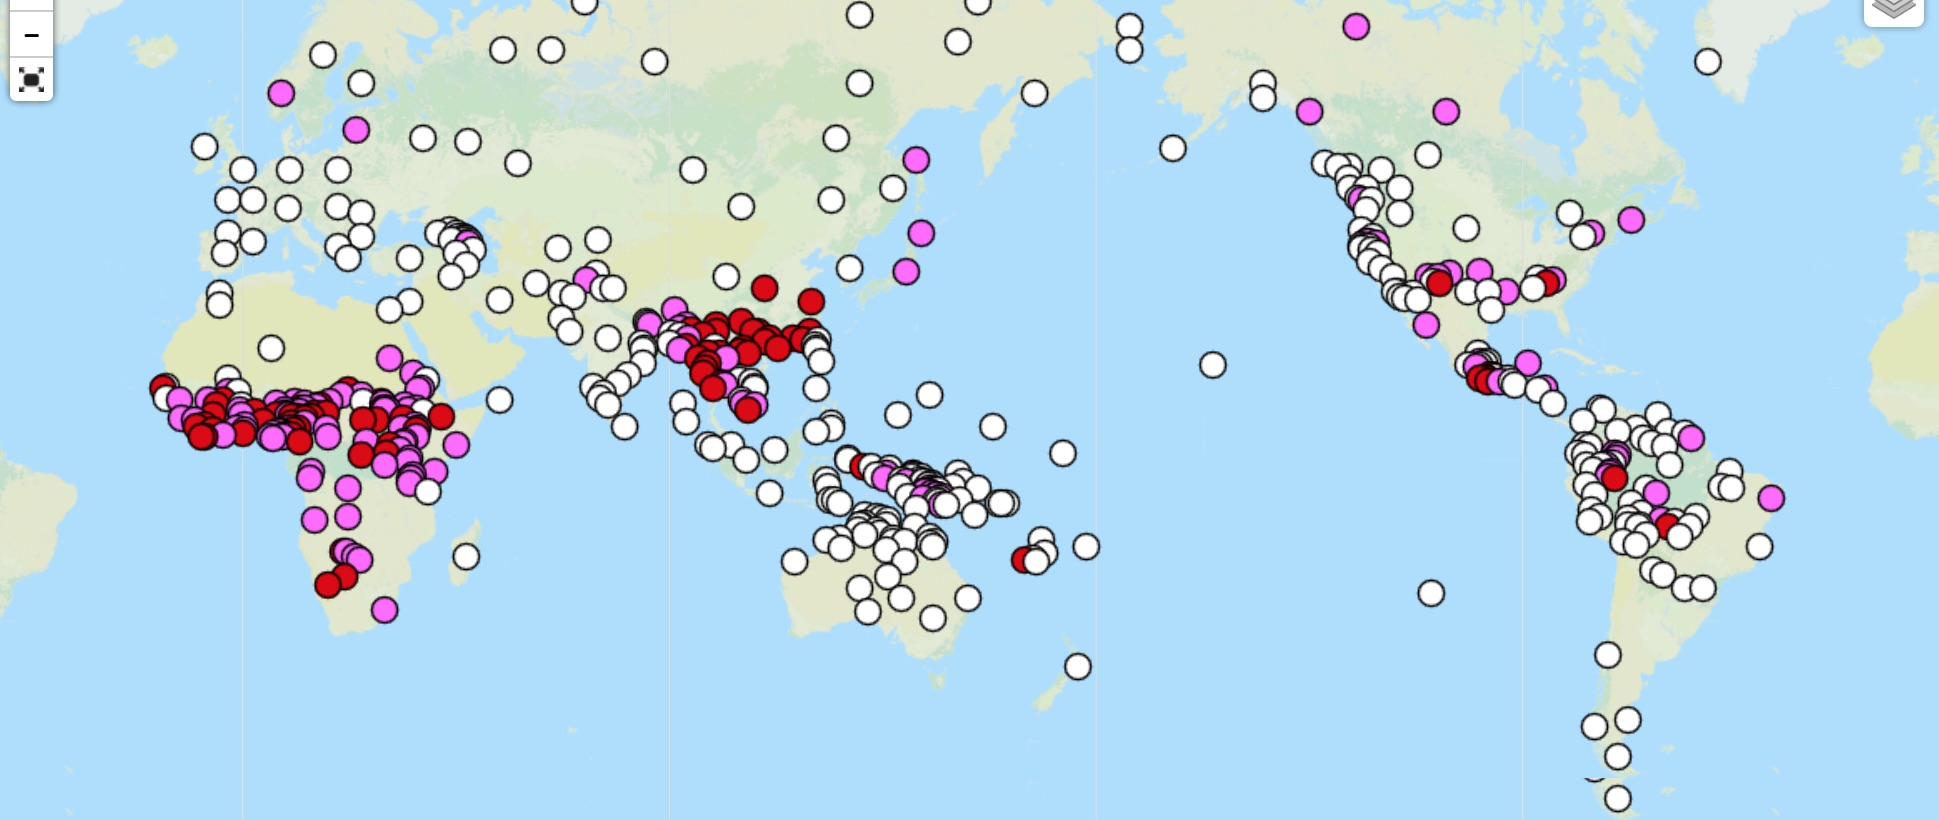
\includegraphics[width=\textwidth]{figures/collins_fig2.jpg}
\caption{Map of the distribution of complex tonal languages (shown in red), simple tonal languages (pink) and non-tonal languages (white) in WALS \citep{Maddieson2013}.}
\label{fig:collins:1}
\end{figure}


% \begin{figure}
% 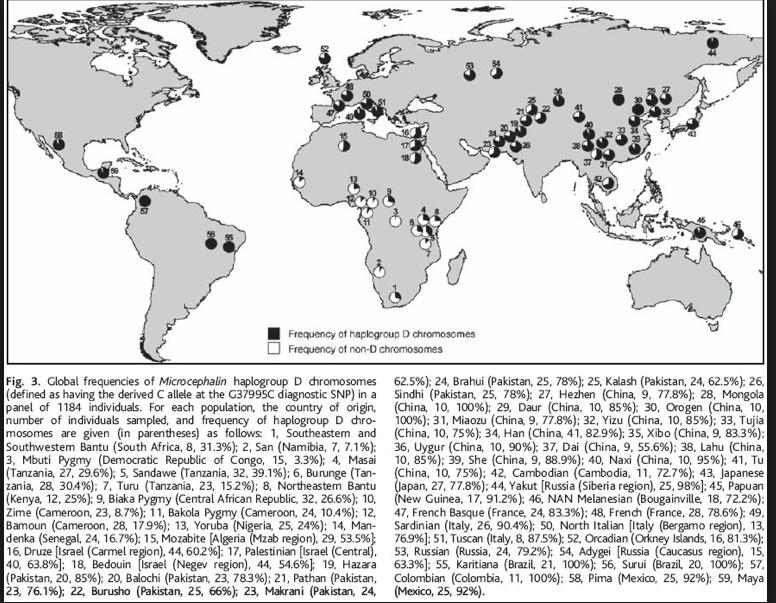
\includegraphics[width=\textwidth]{figures/collins_fig1.jpg}
% \caption{map of the distribution of the derived allele of \textit{microcephalin}.}
% \label{fig:collins:2}
% \end{figure}


\largerpage
Picking two genes to focus on because they occur in the same regions as tone, itself a very spatially clustered linguistic feature, automatically makes this correlation better than most randomly selected correlations between genes and linguistic features.  This makes the fact that this correlation is in the top 97.3\% of gene-feature correlations unimpressive, as all this means is that Dediu and Ladd’s ability to spot visual resemblance between two geographical distributions does better than 97.3\% of selecting completely randomly chosen geographical distributions.  



\is{ASPM} \is{microcephalin} The two genes \textit{ASPM }and \textit{Microcephalin} had no particular reason to be tested, as their effect on cognition was unclear at the time \citep{Dediu2007,Mekel-Bobrov2007}.  If there were an experiment that showed that people with the relevant alleles of \textit{ASPM} or \textit{Microcephalin} were better at tasks involving processing tone, then there would be a reason for studying it.  Interestingly, since the publication of Dediu and Ladd’s paper in 2007, there was a study by \citet{Wong2012} that found that people with the derived allele of \textit{ASPM} were better than those with the ancestral allele at a tone perception task.  This would be an important vindication of their choice of these two genes, although a remarkable fluke given that there was nothing else that Dediu and Ladd knew about \textit{ASPM }that could have led them to hypothesise this.  However, there are two reasons why \citeauthor{Wong2012}’s study cannot be taken as support for Dediu and Ladd’s claim.  The first is that the result of their experiment went in the opposite direction to that predicted by Dediu and Ladd; the ancestral allele is the one that is found in regions with tonal languages, not the derived allele.  The second reason is that \citeauthor{Wong2012}’s sample only contained thirty-two participants.  This makes it quite possible that their result is a false positive.      



For me, the lack of a proper justification for why they chose those genes makes much of their argument invalid, no matter how statistically well supported the correlation is, such as the comparison with other gene-feature correlations, or even the fact that it survives the controls for language family and geography.  However, it is still an interesting question why the correlation is that strong, and why it continues to be after using a Mantel test. \is{Mantel testing}



% In order to answer this, I looked at a different type of genetic marker, mitochondrial DNA.  The purpose of doing this was to find out how often a randomly selected mitochondrial DNA haplogroup will correlate with tone (either presence of tone or number of tones) in a Mantel test after controlling for language relatedness and geographical distance.  Mitochondrial DNA is a good tracker of human migrations, as it is transmitted from the mother to children, and hence one can use a particular type of mitochondrial DNA (a haplotype) to trace back where one's maternal ancestors have come from.  A mitochondrial DNA haplogroup can have a historically meaningful distribution, then, which is likely in some cases to correlate with the distribution of tonal languages.  There is also the intriguing possibility that if tone was carried by migration of people, such as the spread of Han people in China, that particular maternal lineages may correlate with the presence of tone and illuminate the way that it has spread.
Could correlations like that emerge because of the way that genetic variants and linguistic features \is{bilingualism}
cluster together due to linguistic areality? Southeast Asia in particular is one area of the world where there has been widespread bilingualism and sharing of linguistic properties such as tone \is{tone} \is{transmission!horizontal}
across language families \citep{EnfieldAreal2005}. To the extent that this was accompanied by gene flow
between these populations, a correlation could emerge between tone and particular genetic variants
beyond that predicted by language family boundaries and geographical distance. In order to answer
this, I looked at mitochondrial DNA haplogroups, in order to see how often a randomly selected
haplogroup would correlate with tone (either presence of tone or number of tones) in a Mantel test
after controlling for language relatedness and geographical distance. Mitochondrial DNA is a good
tracker of human migrations, as it is transmitted to children from their mother, and hence one can\is{mitochondrial DNA}\is{haplogroup} use a particular type of mitochondrial DNA (a haplotype) to trace back where ones maternal
ancestors have come from. A mitochondrial DNA haplogroup can have a historically meaningful
distribution, then, which is likely in some cases to correlate with the distribution of tonal
languages. There is also the intriguing possibility that if tone was carried by migration of people,
such as the spread of Han people in China, that particular maternal lineages may correlate with the
presence of tone and illuminate the way that it has spread.





% I collected frequencies of mitochondrial DNA haplogroups from 74 populations in Africa and Eurasia, representing 26 different language families (Collins in preparation).  The populations are shown in \figref{fig:collins:3}, along with an example of a haplogroup, HV.  The mitochondrial DNA haplogroups numbered 252, of all levels of specificity available in the literature (from tables of haplogroup frequencies rather than from the nucleotide sequence data). 

% \begin{figure}
%  \caption{Locations of the populations sampled in this paper, along with an example of a particular mtDNA haplogroup (HV).  Populations in red have a population frequency of haplogroup HV above 30\%; populations in dark blue have a frequency above 0\%; and populations in light blue do not have haplogroup HV.}
%  \label{fig:collins:3}
% \end{figure}



% Mitochondrial DNA haplogroups range in levels of specificity; for example, I may belong to haplogroup H1, and this will mean that more generally I belong to H, and even more generally HV, and so on, back to the haplogroup M and eventually back to L0, which all modern humans belong to.  



% The frequencies of haplogroups were therefore calculated using a family tree of mtDNA: the frequency of H1 in a population contributes to the frequency of H, and so on upwards in the phylogeny, using .  \todo{some content missing here}


I collected frequencies of mitochondrial DNA haplogroups from 74 populations in Africa and
Eurasia, representing 26 different language families. A total of 252 mtDNA haplogrups were used,
of all levels of specificity available in the literature (from tables of haplogroup frequencies rather
than from the nucleotide sequence data).

\is{mitochondrial DNA} \is{phylogeny} Mitochondrial DNA haplogroups range in levels of specificity; for example, a person may belong to
haplogroup H1, and this will mean that more generally they will belong to H, and even more
generally HV, and so on, back to the haplogroup M and eventually back to L0, which all modern
humans belong to. The frequencies of haplogroups were therefore calculated using a family tree of
mtDNA: the frequency of H1 in a population contributes to the frequency of H, and so on upwards
in the phylogeny, using the phylogeny from \citet{vanOven2009}.



\is{tone} \is{Mantel testing} \is{Haversine formula} The conclusion of this analysis is that mitochondrial DNA is a
good predictor of the distribution of tonal languages, and remains so after applying statistical
controls for relatedness and geographical distance (although I should emphasise that these are not
exactly the same as the controls that Dediu and Ladd used).  Each haplogroup was tested in a partial Mantel test with number of tones that languages have, controlling for language family (here, pairs of languages are coded as 1 for being in the same family and 0 for being in different families) and geographic distance calculated using the Haversine formula (this does not take landmasses into account or geographical barriers).  26 out of 206 haplogroups correlate with number of tones in this test, meaning that there is a 12\% chance that a neutral genetic marker will correlate with number of tones after apparently factoring out historical relationships between languages.  This means that their result does not in fact reach conventional significance (i.e. there is a much greater than 5\% chance of their result given the null hypothesis).  This result is 14\% if instead of number of tones languages are simply coded for presence or absence of complex tone (namely having more than two tones), as Dediu and Ladd did.  



Overall difference between populations in the frequencies of haplogroups, calculated simply as Manhattan distance of these frequencies, also turns out to correlate with number of tones after controls for language relatedness and geography (r=0.18, p{\textless}0.001).  The most impressive claim in their paper, therefore – that after controlling for language history their correlation holds – in fact turns out to be explicable in terms of the way that neutral genetic markers and linguistic features cluster together, perhaps helped by migration between populations. 



None of this invalidates the general hypothesis that genes can affect the structure of languages.  There is probably genetic variation in linguistic abilities within populations, and when these differences can be between populations too, then one would expect that these can affect language production and what type of linguistic structures catch on in a community.  The way to study these, however, is to start from a hypothesis about genes themselves, and then to test the cross-linguistic prediction.  There may be variation in places such as China in ability to process tone, just as there are genetic differences in people’s ability to process musical pitch; studies of speech disorders may reveal some examples.  It is even possible that genes for processing pitch in language may have undergone natural selection, given the communicative importance of intonation in most languages \citep{Cruttenden1997} and commonalities across
languages such as the use of rising intonation for questions and falling intonation for assertions \citep{Dryer2013polarquestions}. 



Work currently being done by Dediu and Moisik on differences in the vocal tract between populations is one example of work on genetic influences on language which begins from a physiological mechanism and makes a cross-linguistic prediction (Dediu, this volume).  This type of work may be successful, as it is quite plausible that the morphology of the vocal tract varies between populations and makes certain phonemic distinctions more likely to occur in some populations than others.  But the particular case of tone, ASPM and Microcephalin is probably misguided.



\section{Tone and climate}

\is{tone} \is{climate} \citet{Everett2015} find a correlation between humidity and complex tone, a correlation that holds up within different families and parts of the world.  They suggest that dry air is known to affect the larynx and make precise phonation more difficult, precisely the kind of thing that really could (in principle) affect the way that people use a tonal language.



The number of tones that languages use correlates with humidity within five different global areas (Africa, Eurasia, South America, North America, and the Pacific), and within four different language families (\ili{Sino-Tibetan}, \ili{Austro-Asiatic}, \ili{Afro-Asiatic}, \ili{Niger-Congo}).  This is better statistical support than even for word order universals, which despite having some support when sampling from different macro-areas \citep{Dryer1992greenbergian} do not seem to hold consistently within large language families \citep{Dunn2011}.     



In addition, the experimental evidence that they cite showing that dry air has an effect on the larynx raises a host of linguistic questions that are worth exploring anyway, even without this global correlation between dryness and lack of tone.  Do speakers of \ili{Cantonese} alter their use of tone in dryer conditions, for example?  This may be a realistic expectation, if the effect of desiccated air on the larynx is as strong as it is reported in experiments.  China is a natural testing ground for work of this kind, given that varieties of \ili{Chinese} vary in their number of tones and in their climatic conditions.  



However, as I argue in a
response to their paper in the inaugural issue of the \textit{Journal of Language Evolution} \citeyear{CollinsInPress}, there is
an important confound in the correlation between complex tone and humidity.  In brief, there are a lot more languages in humid environments than in non-humid environments (the correlation is Pearson’s $r$=0.31, p{\textless}0.001).  If tone had developed purely at random in the world’s languages, they would still be expected to be found in the more humid places.  I show this in a series of simulations in my paper, in which tone develops in a random set of languages and then spreads by language contact to a set of neighbours.  In all models, it is very likely (between 50 and 83\% depending on the parameters) that tone will correlate with humidity even after using the same controls for language family and the random independent samples test that \citeauthor{Everett2015} employ. 



  
%%please move the includegraphics inside the {figure} environment
%%\includegraphics[width=\textwidth]{CollinsDependencies-img4.png}
 


% \begin{figure}
% \caption{a map of language density, with each star proportional to the number of languages in a 100 km radius, using data from Glottolog \citep{Nordhoff2014}.}
% \label{fig:4}
% \end{figure}


Another finding of \citeauthor{Everett2015}’s paper is that number of tones correlates within large language families, such as \ili{Sino-Tibetan} (Pearson’s $r$=0.16, p{\textless}0.01) and \ili{Niger-Congo} (Pearson’s $r$=0.3, p{\textless}0.001).  However, the major confound here is once again language contact. \is{language contact} \ili{Sino-Tibetan} languages also have fewer tones when they are near to generally non-tonal \ili{Indo-European} languages, and have more tones when near highly tonal \ili{Hmong-Mien} languages.  \ili{Niger-Congo} languages similarly lose tones near non-tonal (or low-tonal) families such as \ili{Nilo-Saharan} and \ili{Afro-Asiatic}.  This matters because speakers of non-tonal languages may be affecting the tonal systems of \ili{Niger-Congo} and \ili{Sino-Tibetan} languages.  An example is \ili{Swahili}, which has no tones despite being a \ili{Bantu} language, most of which have several tones.  The reason for this is probably influence from \ili{Arabic} and its use by Arab traders.  A phylogenetic analysis of \ili{Sino-Tibetan} and \ili{Niger-Congo} shows that these languages have a strong tendency to lose tones as they move towards non-tonal languages in other families, in accordance with this prediction \citep{CollinsInPress}. \is{language contact} \is{phylogeny}



The causal mechanism is
intriguing and worth testing in naturalistic contexts, such as in conversations in different \ili{Chinese}
varieties.  However, language contact should be considered a serious confound in the way that it can create a positive global correlation between humidity and complex tone, including after controlling for language family, and even within families.



\section{Conclusions}



\is{language contact} When trying to find dependencies between linguistic traits, one should be aware of various sources of non-independence of data points when testing a correlation.  Languages are related to each other by common descent in language families, and hence there needs to be a control for relatedness.  But they also influence each other by language contact, and this causes traits such as tone, which spread a long way by contact through languages such as those in Southeast Asia, to form spurious correlations with other traits found in those regions.  



With regard to other dependencies discussed in this volume, there are perhaps other unexpected sources of non-independence of data points that need to be taken into account.  A particularly subtle form is the historical non-independence of individual linguistic constructions.  An example is the way that adpositions often derive from verbs or nouns, and hence correlate in their ordering with verb-object order or genitive-noun order (depending on their source) \citep{Aristar1991}.  Prepositions in \ili{Mandarin}, for example, are thus not historically independent from verbs, as they share a common ancestor.  This is a more subtle kind of Galton’s problem \is{Galton's problem} meaning that the correlation between verb-object ordering and having prepositions in many languages cannot be deduced to be causal, if the word forms for prepositions are in fact derived from verbs.  It may be taking it to an extreme to argue that word order correlations are simply due to processes such as grammaticalization, \is{grammaticalization} as some people have argued \citep{Aristar1991}, and which is discussed by Cristofaro (2017, in this volume).  But it is a surprisingly difficult point to convey to people, who insist that grammaticalization may just be the way that functionally motivated \is{functional principles} word order correlations can arise.  They are missing the point, which is that if they wish to claim a functional motivation, they must first deal with Galton’s problem – in this case, in its more subtle form of the common ancestry of constructions, which however is no less real than the common ancestry of whole languages.



\is{meme} This last point in particular stresses the history of individual constructions and properties of languages, for which I think the word ``meme" is an appropriate cover term \citep{Dawkins1976}. The way that individual memes can travel between languages and have interconnected ancestries of their own creates problems for inferring causal dependencies.  Many of these points are echoed in this volume, as well as in recent work by Enfield such as \textit{Natural Causes of Language }\citep{EnfieldNaturalCauses2014}.  He discusses the fact that behind the illusion of whole languages replicating and dividing into family trees, and behind the illusion of whole linguistic systems, lie instead linguistic replicators which have their own histories but nevertheless need to interact to produce functionally coherent systems. Richard Dawkins makes this point as succinctly as anyone and is arguably its originator, having argued it forcefully for the case of genes building organisms, and then in coining the word ``meme" for similar processes acting in cultural evolution.  To quote from his foreword to Susan Blackmore’s \textit{The Meme Machine }\citep{Blackmore1999}: \is{meme}



``Every gene in a gene pool constitutes part of the environmental background against which other genes are naturally selected, so it’s no wonder that natural selection favors genes that ‘cooperate’ in building these highly integrated and unified machines called organisms.  Biologists are sharply divided between those for whom this logic is as clear as daylight, and those (even some very distinguished ones) who just do not understand it – who naively trot out the obvious cooperativeness of genes and the unitariness of organisms as though they somehow count against the ‘selfish gene’ view of evolution… By analogy with coadapted gene complex, memes, selected against the background of each other, ‘cooperate’ in mutually supportive memeplexes…"



Although Enfield does not use the word ``meme" to describe these replicators, the influence of the idea on this view of language is clear.  For me, the additional relevance of the ``meme" idea is to think in terms of individual properties of language and the way that they can be transmitted by horizontal transfer, and themselves have interconnected ancestries, as genes can, and these need to be understood in order to where the genuine functional dependencies are. \is{transmission!horizontal}



{\sloppy
\printbibliography[heading=subbibliography,notkeyword=this]
}

% \todo[inline]{The references are in a very bad shape and far away from the Unified Stylesheet for linguistics. The author should be asked to provide correct references respecting the guidelines. This means adding first names, conforming the order of elements and not using 'et al.' in the list of references. A bibtex file is of course also a possibility}

% 
% A. R. Aristar. 1991. On Diachronic Sources and Synchronic Patterns: An investigation into the origin of linguistic universals.  Language, 67: 1{}-33 (1991).]{A. R. Aristar, On Diachronic Sources and Synchronic Patterns: An investigation into the origin of linguistic universals.  Language 67: 1-33 (1991).}
% 
% Atkinson, Quentin. 2011. Phonemic Diversity Supports a Serial Founder Effect Model of Language Expansion from Africa.  \textit{Science} 332, 346-349.
% 
% 
% 
% Blackmore, S. 1999. The Meme Machine.  Oxford:Oxford University Press.
% 
% 
% Collins, J. in press.  The Role of Language Contact in Creating Correlations Between Humidity and Tone.  \textit{Journal of Language Evolution}.
% 
% 
% 
% Cruttenden, A. 1997. Intonation (Second Edition), Cambridge: Cambridge University Press.
% 
% 
% 
% Dediu, D. 2007. Non-spurious correlations between genetic and linguistic diversities in the context of human evolution. PhD Thesis  University of Edinburgh, Edinburgh, UK.
% 
% 
% 
% Dediu Dan and D. R. Ladd. 2007. Linguistic tone is related to the population frequency of the adaptive haplogroups of two brain size genes, \textit{ASPM} and \textit{Microcephalin}\textit{.  PNAS} \textbf{104(26)}:10944–10949 
% 
% 
% 
% Donegan, P. and D. Stampe. 1983. Rhythm and the holistic organisation of language structure.  In J. F. Richardson, M. Marks, A. Chukerman, (eds.), Papers from the Parasession on the Interplay of Phonology, Morphology, and Syntax, 337-353. Chicago: Chicago Linguistic Society.
% 
% 
% 
% M. Donohue, \textit{et al.,} World Phonotactics Database.  (Department of Linguistics, The \ili{Australian} National University, Canberra, 2013) \url{http://phonotactics.anu.edu.au}.  Accessed 15/6/2015.
% 
% 
% 
% Dryer, M. S. 1992. The Greenbergian Word Order Correlations.  \textit{Language} \textbf{68}, 81-138 (1992).
% 
% 
% 
% Dryer, M. S. 2013. Polar Questions. In M. S Dryer, Matthew S. \& M. Haspelmath, eds., The World Atlas of Language Structures Online. Leipzig: Max Planck Institute for Evolutionary Anthropology 2013. (Available online at http://wals.info/chapter/116, Accessed on 2016-01-26.)
% 
% 
% 
% Dunn, M., S. Greenhill, S. C. Levinson, R. D. Gray. 2011. Evolved Structure of Language Shows Lineage-Specific Trends in Word Order Universals.  \textit{Nature} \textbf{473}, 79-82.
% 
% 
% 
% Enfield, N. J. 2005.  Areal Linguistics and Mainland Southeast Asia.  \textit{Ann. Rev. Anth.} \textbf{34}, 181-206.
% 
% 
% 
% Enfield, N. J. 2014. Natural Causes of Language: Frames, Biases, and Cultural Transmission. Berlin: Language Science Press.
% 
% 
% 
% Evans, P.  et al. 2005. Microcephalin, a Gene Regulating Brain Size, Continues to Evolve Adaptively in Humans.  \textit{Science} \textbf{309}\textbf{:}1717-1720 (2005).
% 
% 
% 
% Everett, C., D. Blasi, S.G. Roberts. 2015. Climate, Vocal Folds and Tonal Languages: Connecting the Physiological and Geographic dots.  \textit{Proc. Natl Acad. Sci. USA} \textbf{112}, 1322--1327.
% 
% 
% 
% T. L. Gottfried, \textit{et al.}, Effect of Linguistic Experience on the Identification of \ili{Mandarin} \ili{Chinese} Vowels and Tones.  \textit{Journal of Phonetics} \textbf{25}, 207-231 (1997).  
% 
% 
% 
% H. Hammarström, \textit{et al.,} Glottolog 2.0.  (Max Planck Institute for Evolutionary Anthropology, Leipzig, 2014).
% 
% 
% 
% D. R. Ladd,S. G. Roberts, D. Dediu, Correlational studies in typological and historical linguistics. \textit{Annual Review of Linguistics }\textbf{1:}221-241. doi:10.1146/annurev-linguist-030514-124819. (2015)
% 
% 
% 
% I. Maddieson, Tone. In M. S Dryer, Matthew S. \& M. Haspelmath, eds., The World Atlas of Language Structures Online. (Leipzig: Max Planck Institute for Evolutionary Anthropology 2013). (Available online at http://wals.info/chapter/116, Accessed on 2016-01-26.) 
% 
% 
% 
% N. Mekel-Bobrov, et al., Ongoing Adaptive Evolution of ASPM, a Brain Size Determinant in Homo sapiens. \textit{Science} \textbf{309}: 1720-1722 (2005).
% 
% 
% 
% N. Mekel-Bobrov, et al., The ongoing adaptive evolution of \textit{ASPM} and \textit{Microcephalin} is not explained by increased intelligence.  \textit{Hum \ili{Mol} Genet} \textbf{16}:600–608.  (2007)  
% 
% 
% 
% S.G. Roberts, J. Winters, Linguistic diversity and traffic accidents: Lessons from statistical studies of cultural traits. PLoS One, 8(8): e70902. doi:doi:10.1371/journal.pone.0070902.  (2013)
% 
% 
% 
% P.C.M.Wong, B.Chandrasekaran, J.Zheng, The derived allele of ASPM is associated with lexical tone perception.  \textit{PLoS ONE} \textbf{7(4)}: e34243 
% 
% 
% 
% \url{http://journals.plos.org/plosone/article?id=10.1371/journal.pone.0034243} (2012).
% 
% 
% 
% S. Yiu, S. Matthews, Correlations between tonality and word order type.  The 10th Biennial Conference of the Association for Linguistic Typology (ALT 10), (Leipzig, Germany, 15-18 August 2013).

\end{document} 